% ***************************** MAIN FILE **********************************

\documentclass[12pt]{scrreprt}           % Art des zu erstellenden Dokuments
% bei zweiseitigem Druck twoside-Option oder book-Klasse verwenden

% ****************************** PREAMBLE **********************************
% **************************** PACKAGE SETUP *******************************
\usepackage[ngerman]{babel}          % Lokalisierung von Typographie, Silbentrennung, etc.

\usepackage{ucs}                     % Erweiterte Unterstützung von UTF-8-Kodierung
\usepackage[utf8x]{inputenc}         % Unterstützung von UTF-8 in Eingabe-Dateien
\usepackage[T1]{fontenc}             % Zeichensatzkodierung von LaTeX (Cork-Kodierung)
\usepackage{helvet,courier,mathptmx} % Verwendete Schriftarten

\usepackage[headsepline, plainheadsepline, plainfootsepline] {scrlayer-scrpage}

\usepackage{amsmath}                 % Mathematische Infrastruktur für LaTeX der AMS
\usepackage{amsfonts}                % Mathematische Schriftarten
\usepackage{amssymb}                 % Mathematische Symbole
\usepackage{amsthm}                  % Erweiterung der Theorem-Umgebungen
\usepackage[]{units}				 % für \unit-Befehl
%\usepackage[amssymb]{siunits}		 % für SI-Einheiten (amssymb definiert den Befehl \square des amssymb Packages um. Ist dies nicht gewünscht kann die Option squaren verwendet werden. Dann muss für die SI-Einheiten \squaren anstatt \square verwendet werden.)

%\usepackage{fancyhdr}               % Erweiterte Konfiguration von Kopf/Fußzeile
\usepackage{hyperref}                % Querverweise, Hyperlink, pdf-Konfiguration, etc.

\usepackage{float}                   % Selbstdefinierte Floating-Umbgebungen
\usepackage{tabularx}                % Tabellen mit einstellbarer Spaltenbreite
\usepackage[labelfont=bf]{caption}   % Anpassen der Abbildungs- und Tabellenbeschriftungen

\usepackage{algpseudocode}           % Algorithmen als Pseudocode (basiert auf algorithmicx)
\usepackage{listings}                % Quellcode-Satz (z.B. mit Syntax-Hervorhebung)
\lstset { %
    language=Python,
    backgroundcolor=\color{black!5}, % set backgroundcolor
    basicstyle=\footnotesize,        % basic font setting
}

\usepackage[pdftex,
%draft							     %Figures werden nur als Platzhalter eingeblendet
]{graphicx}						     % Erweiterte Unterstützung von Graphiken
\usepackage{textpos}                 % Beliebig platzierte Textboxen
\usepackage{xcolor}                  % TeX-Engine-unabhängige Definition von Farben
\usepackage{acronym}


\usepackage{pdfpages}

\usepackage[numbers]{natbib}         % Weiter Optionen für die Bibliographie
\usepackage{todonotes}
\usepackage{tabulary}
\usepackage{IEEEtrantools}
\usepackage{multicol}
\usepackage{graphicx}
\usepackage{enumitem}
\usepackage{tabularx}


% ****************************** TOP MATTER ***********************************
\newcommand{\studenteins}{Erkan Garan}           % Name
\newcommand{\matrNumbereins}{70467533}              % Matrikelnummer
\newcommand{\studycourse}{Informatik}           % Studiengang

\newcommand{\supervisor}{Prof. Dr. Claus Fühner, Stefan Jung} % Betreuer
\newcommand{\institution}{Ostfalia Hochschule} % Hochschule
\newcommand{\subinstitution}{Hochschule Braunschweig/Wolfenbüttel}
\newcommand{\faculty}{Informatik}               % Fachbereich
\newcommand{\toponym}{Wolfenbüttel}                 % Ort

\renewcommand{\subject}{Bachelorarbeit}  % Art/Thema der Arbeit
\newcommand{\titel}{{Entwurf eines Modells für ein unterstützendes KI-System zur Bewertung von Anwendungsregeln}} % Titel der Arbeit
\newcommand{\subtitel}{} % Untertitel
\newcommand{\graduation}{Bachelor of Science} % Angestrebter Titel (nur bei Abschlussarbeiten, sonst leer lassen/auskommentieren)

\newcommand{\keywords}{{}} % Stichworte (durch Komma getrennt)


% **************************** HYPERREF SETUP *******************************
\definecolor{linkcolor}{rgb}{1,0.5,0}
\hypersetup
{
bookmarks=true,                        % Lesezeichen im PDF erzeugen
bookmarksopen=true,                    % Lesezeichen im PDF sofort anzeigen
backref=true,                          % Rückverweise im Literaturverzeichnis
colorlinks=true,                       % Farbige Verweise
%hidelinks = true,                      % Verweise verbergen (entfernt Farbe und Rahmen)
pdfstartview={FitH},                   % Ansicht des PDFs beim öffnen
pdftitle={\titel},                     % Title des PDFs
pdfauthor={\author , \supervisor},     % Autor des PDFs
pdfsubject={\subject},                 % Thema des PDFs
%pdfcreator={Creator},                 % Erzeuger des Dokuments (Anwendungsprogramm)
%pdfproducer={Producer},               % Ersteller des PDFs (Programm/Bibliothek/Skript)
pdfkeywords={\keywords},               % Stichwörter zum PDF
linkcolor=linkcolor,                   % Farbe von Querverweisen
citecolor=green,                       % Farbe von Zitaten
filecolor=magenta,                     % Farbe von Verweisen auf Dateien
urlcolor=cyan                          % Farbe von URLs
}
% Weitere Optionen: http://www.tug.org/applications/hyperref/manual.html

% **************************** LISTINGS SETUP *******************************
\definecolor{keywords}{rgb}{0.5 0 0.3}
\definecolor{comments}{rgb}{0.25,0.5,0.37}
\lstset{ %
  backgroundcolor=\color{white},   % Hintergrundfarbe
  basicstyle=\linespread{0.94}\footnotesize\ttfamily, % Schrifteinstellungen für Quellcode
  breakatwhitespace=false,         % Automatische Zeilenumbrüche nur bei Leer- oder Tabulatorzeichen (Leerraum/whitespaces)
  breaklines=true,                 % Automatische Zeilenumbrüche
  captionpos=b,                    % Beschriftung unten
  commentstyle=\color{comments},   % Schrifteinstellungen für Kommentare
%  deletekeywords={...},            % Bestimmte Schlüsselwörter entfernen
  escapeinside={\%*}{*)},          % Defintion von Escape-Sequenzen
  extendedchars=true,              % Nicht ASCII-Zeichen erlauben
  frame=single,                    % Rahmen um den Quellcode
  keepspaces=true,                 % Einrückungen im Quellcode behalten
  keywordstyle=\bfseries\color{keywords},% Schrifteinstellungen für Schlüsselwörter
  language=java,                   % Programmiersprache des Quellcodes
%  morekeywords={*,...},            % Zusätzliche Schlüsselwörter
  numbers=left,                    % Zeilennummerierung
  numbersep=5pt,                   % Abstand zwischen Zeilennummerierung und Quellcode
  numberstyle=\tiny\color{gray}, % Schrifteinstellungen für Zeilennummern
  rulecolor=\color{black},         % if not set, the frame-color may be changed on line-breaks within not-black text (e.g. comments (green here))
  showspaces=false,                % Leerraum-Zeichen anzeigen
  showstringspaces=false,          % Leerzeichen in Zeichenketten anzeigen
  showtabs=false,                  % Tabulatorzeichen in Zeichenketten anzeigen
  stepnumber=1,                    % Schrittweite bei Zeilennummern
  stringstyle=\color{blue},        % Schrifteinstellungen für Zeichenketten
  tabsize=4,                       % Tabulatorbreite (Anzahl Leerzeichen)
  numberbychapter=false            % Nummeriere Quellcode fortlaufend je Kapitel
}
\renewcommand{\lstlistlistingname}{Quellcodeverzeichnis}
\renewcommand{\lstlistingname}{Quellcode}

\AtBeginDocument{\numberwithin{lstlisting}{section}} % Nummeriere Quellcode fortlaufend je Abschnitt

% ************************** HEADER/FOOTER SETUP ****************************
\pagestyle{scrheadings}

\clearscrheadings				% löscht voreingestellte Stile
\clearscrplain					% löscht voreingestellte Stile

\lohead[\headmark]{\headmark}
\rohead[\pagemark]{\pagemark}

\automark{chapter}

% **************************** GRAPHICX SETUP *********************************
\DeclareGraphicsExtensions{.pdf,.png,.jpg} % bekannte Graphik-Dateiformate (müssen nicht mehr im Dateinamen angegeben werden, also statt "beispiel.png" nur noch "beispiel")
\graphicspath{{./figure/}}   % path to graphics folder, usage {PATH},{ANOTHERPATH}...

% ************************** BIBLIOGRAPHY SETUP ********************************
\bibliographystyle{IEEEtranN}    % Literaturverzeichnis nach IEEE
%\AtBeginDocument{\nocite{*}} % Diese Zeile vor der Abgabe der Arbeit entfernen!

% ****************************** MATH SETUP ************************************
\everymath{\displaystyle}    % Erzwinge \displaystyle für Mathematischen-Modus


% ************************* THEOREMS AND PROOF *********************************
\newtheoremstyle{thesis}     % Name des neuen Theorem-Stils
{3pt}                        % Abstand oberhalb des Theorems
{3pt}                        % Abstand unterhalb des Theorems
{\itshape}                   % Schrifteinstellungen innerhalb des Theorems
{}                           % Einrückung der Theorem-Überschrift
{\bfseries}                  % Schrifteinstellungen für die Überschrift des Theorems
{}                           % Satzzeichen zwischen Überschrift und Theorem-Rumpf
{\newline}                   % Abstand hinter der Überschrift
{}                           % Spezifikation der Überschrift
  
\theoremstyle{thesis}        % Verwende neuen Theorem-Stil

\newtheorem{theorem}{Satz}[section] % neue Theorem-Umgebung: theorem (Satz)
\providecommand*{\theoremautorefname}{Satz} % autoref-Name für theorem

\newtheorem{definition}{Definition}[section] % neue Theorem-Umgebung: definition (Definition)
\providecommand*{\definitionautorefname}{Definition} % autoref-Name für definition

\renewcommand{\qedsymbol}{$\blacksquare$} % Schwarzes Quardrat als Symbol für: q. e. d.
\renewenvironment{proof}[1][\proofname]{{\bfseries #1:}~}{\qed} % "Beweise:" in Fettdruck

% *************************** PSEUDOCODE SETUP ********************************
\floatstyle{boxed}                        % Rahmen für pseudocode-Umgebung
\newfloat{pseudocode}{htbp}{lop}[section] % Definieren pseudocode-Umgebung
\floatname{pseudocode}{Pseudocode}        % Beschrifte pseudocode-Umgebung mit "Pseudocode"

\newcommand{\listofpseudocodename}{Pseudocodeverzeichnis}
\newcommand{\listofpseudocode}{\listof{pseudocode}{\listofpseudocodename}}
\providecommand*{\pseudocodeautorefname}{Pseudocode}

% ******************************* PAGE SETUP **********************************
\textheight23cm
\textwidth14cm
\voffset0cm
\topskip0cm
\topmargin-1.2cm
\headheight1.0cm
\headsep1.5cm
\oddsidemargin1.0cm
\evensidemargin1.0cm
\renewcommand{\baselinestretch}{1.4} 

% Hurenkinder und Schusterjungen verhindern
\clubpenalty = 10000
\widowpenalty = 10000
\displaywidowpenalty = 10000

% Verbesserung der Textsetzung
\tolerance = 1000
\emergencystretch = 20pt

% ******************************** MACROS *************************************
\newcommand{\RR}{\mathbf{R}}
\newcommand{\NN}{\mathbf{N}}
\newcommand{\QQ}{\mathbf{Q}}
\newcommand{\ZZ}{\mathbf{Z}}
\newcommand{\CC}{\mathbf{C}}
\newcommand{\erstelltvon}[1]{\marginpar{\fbox{#1}}}


%%%%%%%%%%%%%%%%%%%%%%%%%%%%%%%%%%%%%%%%%%%%%%%%%%%%%%%%%%%%%%%%%%%%%%%%%%%%%%%
% ************************** BEGINN OF DOCUMENT *******************************
%%%%%%%%%%%%%%%%%%%%%%%%%%%%%%%%%%%%%%%%%%%%%%%%%%%%%%%%%%%%%%%%%%%%%%%%%%%%%%%
\begin{document}
\bstctlcite{IEEEexample:BSTcontrol} 
\pagestyle{plain}

% 
%% *** Titelseite ***
%
\begin{titlepage}
	\vspace*{-3.0cm}
	%Logo international
	%\hspace*{ 9.30cm}
\includegraphics[scale=0.93]{../ostfalia/LSVorlagejpg_klein_int.jpg}\\
	%Logo deutsch
	%\hspace*{10.20cm}
\includegraphics[scale=0.60]{../ostfalia/Ostfalia_LS_RGB_klein.jpg}\\
	\hspace*{ 6.90cm}
\includegraphics[scale=0.93]{../ostfalia/Ostfalia_LS_RGB_klein.jpg}\\
	%Logo ohne Schrift
	%\hspace*{15.00cm}
\includegraphics[scale=0.60]{../ostfalia/Ostfalia_L_RGB_klein.jpg}\\
	%\hspace*{14.30cm}
\includegraphics[scale=0.93]{../ostfalia/Ostfalia_L_RGB_klein.jpg}\\
	\hspace*{-1.00cm}
\includegraphics[scale=1.20]{../ostfalia/Reiter_Wolfen_RGB_174mm.jpg}\\
	
	\hspace*{-0.5cm}{\Large\textsf{Fakultät \faculty}}\\
	
	\hrulefill\\
	
	%-------------------------------------------------------------------------------
	\noindent{\Large\textsf{\studenteins, \matrNumbereins\\}}
	\ifdefined\studentzwei%
	\if\studentzwei\empty
	\else
	{\Large\textsf{\studentzwei, \matrNumberzwei\\}}
	\fi
	
	
	\vspace{2em}
	\textbf{
	\textsf{\huge\titel \\[0.3ex]}}
	\textsf{\hspace*{0.5cm}\large \subtitel \\[0.05cm]}
	
	\vspace{2em}
	\begin{center}
	\ifdefined\graduation%
	\if\graduation\empty%
	\else%
	\textsf{Abschlussarbeit zur Erlangung des akademischen Grades}\\[0.5cm]
	\textsf{\graduation} \textsf{im Studiengang Informatik}\\[0.5cm]
	\textsf{an der \institution}\\[0.5cm]
	\textsf{\subinstitution}
	\fi
	\end{center}
	
	\vspace*{\fill}

 	\enlargethispage{1\baselineskip}
	\hrulefill\\
	\begin{center}
		\textsf{Betreuer: \\  \supervisor}
	\end{center}
	
	\vspace*{\fill}
	
	%-------------------------------------------------------------------------------
	
	\enlargethispage{4\baselineskip}
	\begin{minipage}[b]{0mm}
		\raisebox{24mm}{\hspace*{-1.00cm}
\includegraphics[scale=1.20]{ostfalia/Reiter_szsudwob_RGB_174mm.jpg}}
	\end{minipage}
	
	%*******************************************************************************
	
\end{titlepage}


% ***************************** FRONT MATTER **********************************
\setcounter{page}{1}
\pagenumbering{Roman}
\chapter*{}
\vspace*{0.5cm}
\noindent

Hiermit versicheren wir, dass wir die vorliegende Arbeit selbstständig verfasst und keine anderen als die angegebenen Quellen und Hilfsmittel benutzt haben. Wir versicheren, dass wir alle wörtlich oder sinngemäß aus anderen Werken übernommenen Aussagen als solche gekennzeichnet haben, und dass die eingereichte Arbeit weder vollständig noch in wesentlichen Teilen Gegenstand eines anderen Prüfungsverfahrens gewesen ist.

\vspace{3cm}
\toponym, den \today
%\chapter*{Überblick}
\section*{Kurzfassung}
Anwendungsregeln sind eine besondere Form von Anforderungen. Die Erfüllung dieser Regeln ist essentiell für einen sicheren und zuverlässigen Einsatz von Komponenten, die diese Anwendungsregeln
voraussetzen. Dieser Praxsibericht wird sich mit der Datenanalyse von Projekten der Siemens Mobility GmbH beschäftigen, welche Anwendungsregeln bewertet haben. Ziel der Datenanalyse wird es sein,
die Daten in einer für das Anlernen eines unterstützenden KI-Systems zum Bewerten von Anwendungsregeln geeigneten Form aufzubereiten. Dafür werden Daten von Projekten gesammelt, welche Anwendungsregeln
bewertet haben. Daraufhin muss ermittelt werden, welche Attribute für das Anlernen des KI-Systems relevant sein werden. Mit diesen Erkenntnissen können die Daten dann aufbereitet werden. Das Ergebnis
der Datenaufbereitung wird dann in diesem Praxisbericht dargestellt.

\vfill\vfill\vfill\vfill\vfill\vfill
\section*{Abstract}
Application rules are a special form of requirements. The fulfillment of these rules is essential for the safe and reliable use of components that require these application rules.
This report will deal with the data analysis of projects of the Siemens Mobility GmbH, which have evaluated application rules. The goal of the data analysis will be to
prepare the data in a form suitable for training a supportive AI system, which will be used to evaluate application rules. For this purpose, data will be collected from projects 
that have evaluated application rules. It will then be necessary to determine which attributes will be relevant for training the AI system. With these findings, 
the data can then be prepared. The result of the data preparation is then presented in this report.
\vfill\vfill\vfill\vfill\vfill\vfill
% *************************** TABLE OF CONTENTS *******************************
% ************************* (Inhaltsverzeichnis) ******************************
% Die Auskommentierte Zeile fügt das Inhaltsverzeichnis zum Inhaltsverzeichnis hinzu. Diese Verhalten kann auch über das Paket tocbibind erreicht werden. Allerdings funktioniert das Paket nicht für das Pseudocodeverzeichnis, aus diesem Grund werden die Einträge "manuell" hinzugefügt.

%\phantomsection\addcontentsline{toc}{chapter}{\numberline{}\contentsname}
{
\baselineskip=15pt % Schriftlinien-Abstand 15 pt (nur beim Inhaltsverzeichnis)
\tableofcontents   % Inhaltsverzeichnis einfügen
}
{
\baselineskip=22pt % Schriftlinien-Abstand 22 pt (bei allen anderen Verzeichnissen)

% **************************** LIST OF FIGURES ********************************
% ************************ (Abbildungsverzeichnis) ****************************
\clearpage\phantomsection
%\addcontentsline{toc}{chapter}{\numberline{}\listfigurename}

\listoffigures % Abbildungsverzeichnis einfügen

% **************************** LIST OF TABLES *********************************
%\clearpage\phantomsection\addcontentsline{toc}{chapter}{\numberline{}\listtablename}

%\listoftables % Tabellenverzeichnis einfügen

% ************************** LIST OF PSEUDOCODE *******************************
%\clearpage\phantomsection\addcontentsline{toc}{chapter}{\numberline{}\listofpseudocodename}

%\listofpseudocode % Pseudocodeverzeichnis einfügen

% *************************** LIST OF LISTINGS ********************************
%\clearpage\phantomsection\addcontentsline{toc}{chapter}{\numberline{}\lstlistlistingname}

%\lstlistoflistings % Quellcodeverzeichnis einfügen
}
\addchap{Abkürzungsverzeichnis}

\begin{acronym}
	\acro{CRISP-DM}[CRISP-DM]{Cross Industry Standard Process for Data Mining}
	\acro{DOORS}[DOORS]{IBM Rational DOORS}
	\acro{DXL}[DXL]{DOORS Extension Language}
\end{acronym}




% ***************************** MAIN MATTER ***********************************
\pagenumbering{arabic}

\chapter{Einleitung}
\label{chap:einleitung}
\erstelltvon{student 1}
Worum geht es in Ihrer Arbeit

\section{Motivation}
\label{sec:motivation}
Was ist die Motivation hinter dieser Arbeit

\section{Zielsetzung}
\label{sec:zielsetzung}
Ziele der Arbeit

\section{Aufbau}
\label{sec:aufbau}
Aufbau der Arbeit. Sehr kurz. Kann ist kein muss. \acfi{acfi}


\chapter{Bäume in der Informatik}
\label{chap:kapitel2}

\section{Definition von Bäumen}

Nach Wetherell und Shannon sind Bäume endliche, gerichtete, zusammenhängende, azyklische Graphen \cite[]{q1}. 
Die Besonderheit an einem azyklischen Graph ist, dass dieser keine Zyklen enthält. Bäume bestehen im Grunde genommen 
aus zwei Elementen, nämlich den Knoten und den Kanten. Die Kanten sind gerichtet und verbinden die einzelnen 
Knoten miteinander. Dabei hat jeder Knoten maximal einen Vorgänger, welcher als Vater bezeichnet wird, und null 
bis n viele Nachfolger, welche Kinder genannt werden. Die Wurzel stellt hierbei einen besonderen Knoten dar, da sie der 
einzige Knoten ohne Vorgänger ist. Eine weitere besondere Form von Knoten sind die Blätter. Diese verfügen nämlich über 
keine Kinder \cite{q4}.

\begin{figure}[H]
    \centering
    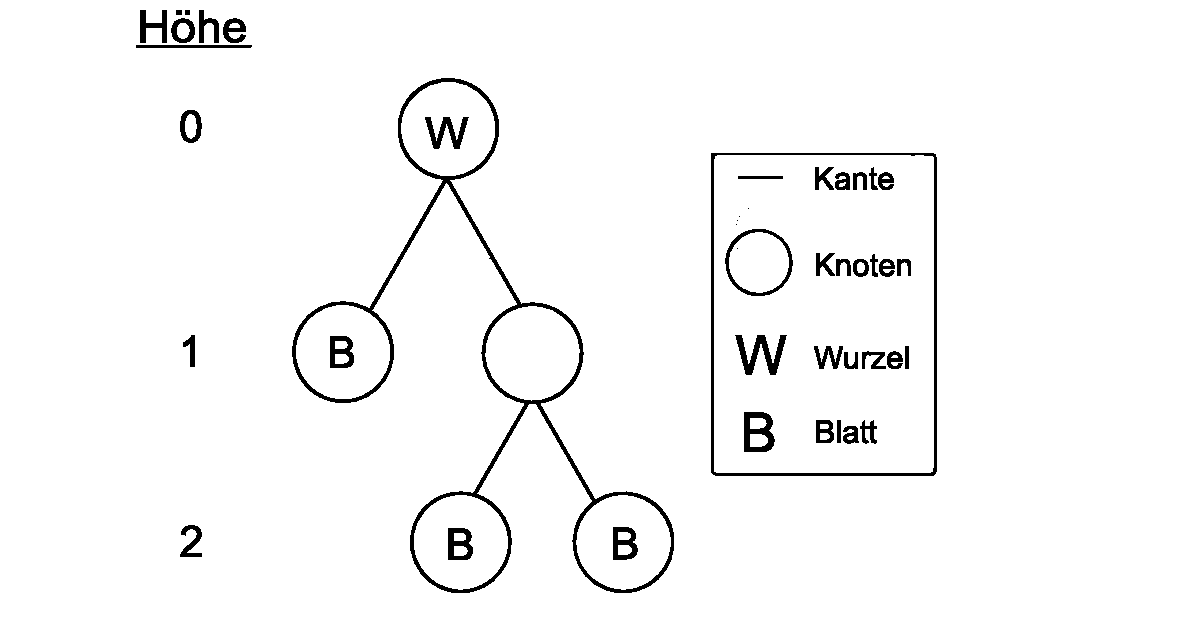
\includegraphics[scale = 0.5]{abbildungen/simple_tree}
    \caption{Einfacher beschrifteter Binärbaum}
    \label{pic:simple_tree} 
\end{figure}

Eine spezielle Form von Bäumen stellen die sogenannten Binärbäume dar. 
Binärbäume sind Bäume, wo jeder Knoten maximal zwei Kinder hat. Abbildung \ref{pic:simple_tree} 
zeigt einen einfachen Binärbaum, wo jedes Element genau beschriftet ist. 

Um jeden Knoten eines Baumes abarbeiten zu können, kann über dem Baum 
traversiert werden. Traversierung bezeichnet das systematische Ablaufen 
von jedem Knoten eines Baumes. Der naive Algorithmus
von Wetherell und Shannon verwendet die sogenannte
Pre-Order-Traversierung. Dabei wird zunächst der Knoten, dann der linke Teilbaum
und zum Schluss der rechte Teilbaum besucht. Hier werden die Väter also vor den
Kindern durchlaufen. Sowohl der verbesserte Algorithmus von Wetherell 
und Shannon als auch der Algorithmus von Reingold und Tilford verwenden hingegen die 
Post-Order-Traversierung. Dabei wird als erstes der linke Teilbaum, dann der 
rechte Teilbaum und dann der Knoten besucht \cite[]{q4}. Bei dieser Art der 
Traversierung werden die Kinder also vor den Väter durchlaufen. Neben diesen Arten
der Traversierung gibt es noch weitere Möglichkeiten, wie über einem 
Baum traversiert werden kann. Diese sind für das Verständnis der hier 
vorgestellten Algorithmen aber nicht notwendig.


\section{Anwendungsgebiete}

Bäume erfahren einen vielfältigen Einsatz in der Informatik, zum Beispiel 
als Datenstruktur, als Syntaxbäume, als Ausdrucksbäume oder auch als 
Entscheidungsbäume.

Ein Baum als Datenstruktur kann beispielsweise dazu verwendet werden, 
um eine Menge von Daten zu sortieren oder in ihnen effizient nach einen 
bestimmten Datensatz zu suchen. So verwendet der Heap-Sort-Algorithmus 
einen Baum zum Sortieren von Daten. Ebenso können Bäume dazu verwendet 
werden, die Syntax von Quellcode zu überprüfen. Ferner werden diese Bäume 
als Syntaxbäume bezeichnet. Zudem werden Bäume verwendet um mathematische 
Ausdrücke auszuwerten. Hierfür wird ein sogenannter Ausdrucksbaum für einen 
gegebenen mathematischen Ausdruck aufgestellt und ausgewertet. In der 
Datenanalyse werden Bäume in Form von Entscheidungsbäumen verwendet. 
Diese werden benutzt um Abhängigkeiten darzustellen. Die Blätter stellen 
Kategorien dar und die Knoten Bedingungen. So können beispielsweise neue 
Datensätze, in Abhängigkeit zu seinen Werten, einer bestimmten Kategorie 
zugeordnet werden.

Auch außerhalb der Informatik werden Bäume häufig verwendet. Sie können 
dazu verwendet werden um zum Beispiel eine Hierarchie eines Unternehmens 
(siehe Abb. 1) dazustellen oder einen Stammbaum einer 
Familie (siehe Abb. 2) \cite[]{q4}.

\todo{Zwei beispielhafte Abbildungen erstellen}


\chapter{Algorithmen zum Zeichnen von Bäumen}
\label{chap:kapitel3}

\section{Naiver Algorithmus von Wetherell und Shannon}

Das Paper “Tidy Drawings of Trees” von Charles Wetherell und Alfred Shannon aus dem Jahre 1979, 
welches im IEEE Trans. Softw. Eng. erschienen ist, handelt von verschiedenen Algorithmen zum Zeichnen von Bäumen.
Der erste Algorithmus, der von den beiden Autoren beschrieben und vorgestellt wird, ist ein naiver Algorithmus 
zum Zeichnen von Bäumen. Dieser Algorithmus soll dabei zwei Anforderungen erfüllen. Die erste Anforderung wird dabei
an die Ästhetik des gezeichneten Baumes gestellt. Alle Knoten, die dieselbe Höhe haben, sollen sich auf einer horizontalen
Linie befinden. Jede Höhe hat dabei eine Linie, auf welcher sich die Knoten befinden sollen und diese Linien sollen alle
parallel zueinander sein. Außerdem soll der Algorithmus beim Zeichnen eines Baumes ein physikalisches Limit einhalten.
Das bedeutet, dass der Algorithmus möglichst schmale Bäume zeichnen soll. Jedoch wird die Höhe des Baumes durch diese Anforderungen
nicht eingeschränkt. Stattdessen bestimmt der Baum selbst seine Höhe. \cite[]{q1}

\subsection{Ablauf}
Bevor die Funktionsweise des Algorithmus beschrieben werden kann, muss die Baumstruktur wie folgt definiert sein: Sie benötigt eine Struktur die symbolisch für ein Knoten des Baums steht. Diese Knoten-Struktur muss hierbei ihren Vater kennen, auf ihre Kinder zugreifen können, ihre Position speichern können. Diese Hilfsvariable wird dazu benutzt, um das nächste abzuarbeitende Kind eines Knoten zu identifizieren. 

In Java könnte diese Struktur beispielsweise wie folgt aussehen:
\begin{lstlisting}
class Knoten {
	Knoten vater;
	Knoten[] kinder;
	int hoehe;
	int x, y;
}
\end{lstlisting}
Dieser Algorithmus besitzt zwei Eingabeparameter: Die Wurzel und Höhe des Baumes. Die Wurzel muss hierbei vom Typ der zuvor definierten Struktur sein. Zu Beginn wird eine Variable definiert: Ein Array (später Positions-Array genannt), die die jeweils nächst freie X-Position einer Ebene des Baums beinhaltet. Hiernach wird über die Baumstruktur der Wurzel, in der Pre-Order-Traversierung, traversiert. Nun werden die X und Y Attribute der Knoten wie folgt bestimmt und gesetzt:

Der derzeitige Knoten bekommt als X-Position den Wert aus dem Positions-Array, in Abhängigkeit von seiner Höhe im Baum. Hiernach wird die Zahl im Positions-Array inkrementiert. Die Y-Position des Knoten wird nun in Abhängigkeit zur Höhe des Knoten mit der folgenden Formel berechnet: y := 2 * Höhe + 1.

Dieses Vorgehen wird nun für alle Knoten in dem Baum wiederholt. 

Nach dem Durchlaufen aller Knoten des Baumes sind alle X und Y-Koordinate gesetzt und der Baum kann gezeichnet werden.

\subsection{Vor- und Nachteile}

\section{Verbesserter Algorithmus von Wetherell und Shannon}

\subsection{Ablauf}

\subsection{Vor- und Nachteile}

\section{Algorithmus von Reingold und Tilford}

\subsection{Ablauf}

\subsection{Implementierung in Java}

\subsection{Vor- und Nachteile}

\subsection{Modifizierung des Algorithmus}


\chapter{Analyse vorhandener Daten}
\label{chap:kapitel4}

Ein Modell, welches beim Data Mining genutzt werden kann, ist das \ac*{CRISP-DM}. Diese Modell definiert das Data Mining als Prozess mit sechs verschiedenen Phasen und kann der 
Abbildung \ref*{fig:CRISP-DM} entnommen werden. Dabei dürfen diese Phasen nicht als starr aufeinander folgend betrachtet werden. Denn auch Erkenntnisse aus nachfolgende Phasen können vorherige Phasen
beeinflussen, was deutlich wird, durch die Pfeile zwischen den Phasen in der Abbildung \ref*{fig:CRISP-DM}. In der ersten Phase, dem Business Understanding, liegt der Schwerpunkt auf dem Verständnis 
der Projektziele aus der Geschäftsperspektive. Mit dem erlangten Wissen daraus, kann eine Data-Mining Problemstellung definiert werden, wie dies in Kapitel \ref*{chap:Zielsetzung} erfolgt ist. 
Die nächste Phase ist das Data Understanding. Diese Phase beschäftigt sich mit der ersten Datenerhebung und dem Aufbau eines Datenverständnisses. Zudem wird in dieser Phase versucht mögliche Probleme 
bei der Qualität der Daten zu identifizieren. Nach der Phase des Data Understandings folgt die Phase der Data Preparation. Während dieser Phase ist das Ziel die Rohdaten so aufzubereiten, dass ein 
Datensatz dabei erstellt wird, der für eine Modellierung geeignet ist \cite[S.5-7]{q8}. Die nächsten drei Phasen beschäftigen sich mit der Modellierung, der Evaluierung von Modellen und dem Einsatz 
eines Modells und gehen somit über die Aufgabenstellung des Praxisprojekt hinaus und werden deshalb im Folgenden nicht berücksichtigt.

\begin{figure}[H]
    \centering
    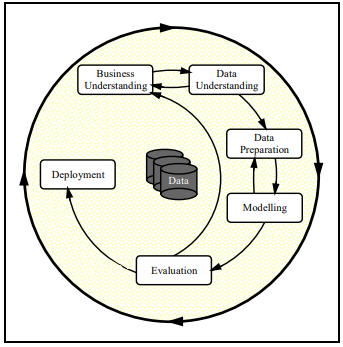
\includegraphics[]{abbildungen/CrispDM.PNG}
    \caption{\ac*{CRISP-DM} Phasen \cite[S.5]{q8}}
    \label{fig:CRISP-DM}
\end{figure}



% ***************************** BIBLIOGRAPHY **********************************
\baselineskip=14pt
\clearpage
\phantomsection
\addcontentsline{toc}{chapter}{\protect\numberline{}\bibname}
\bibliography{bib/thesis}

% ******************************* APPENDIX ************************************
\appendix
\chapter{Anhang A}
\label{chap:anhang_a}

\begin{figure}[ht]
    \centering
    \begin{minipage}[t]{0.45\linewidth}
        \centering
        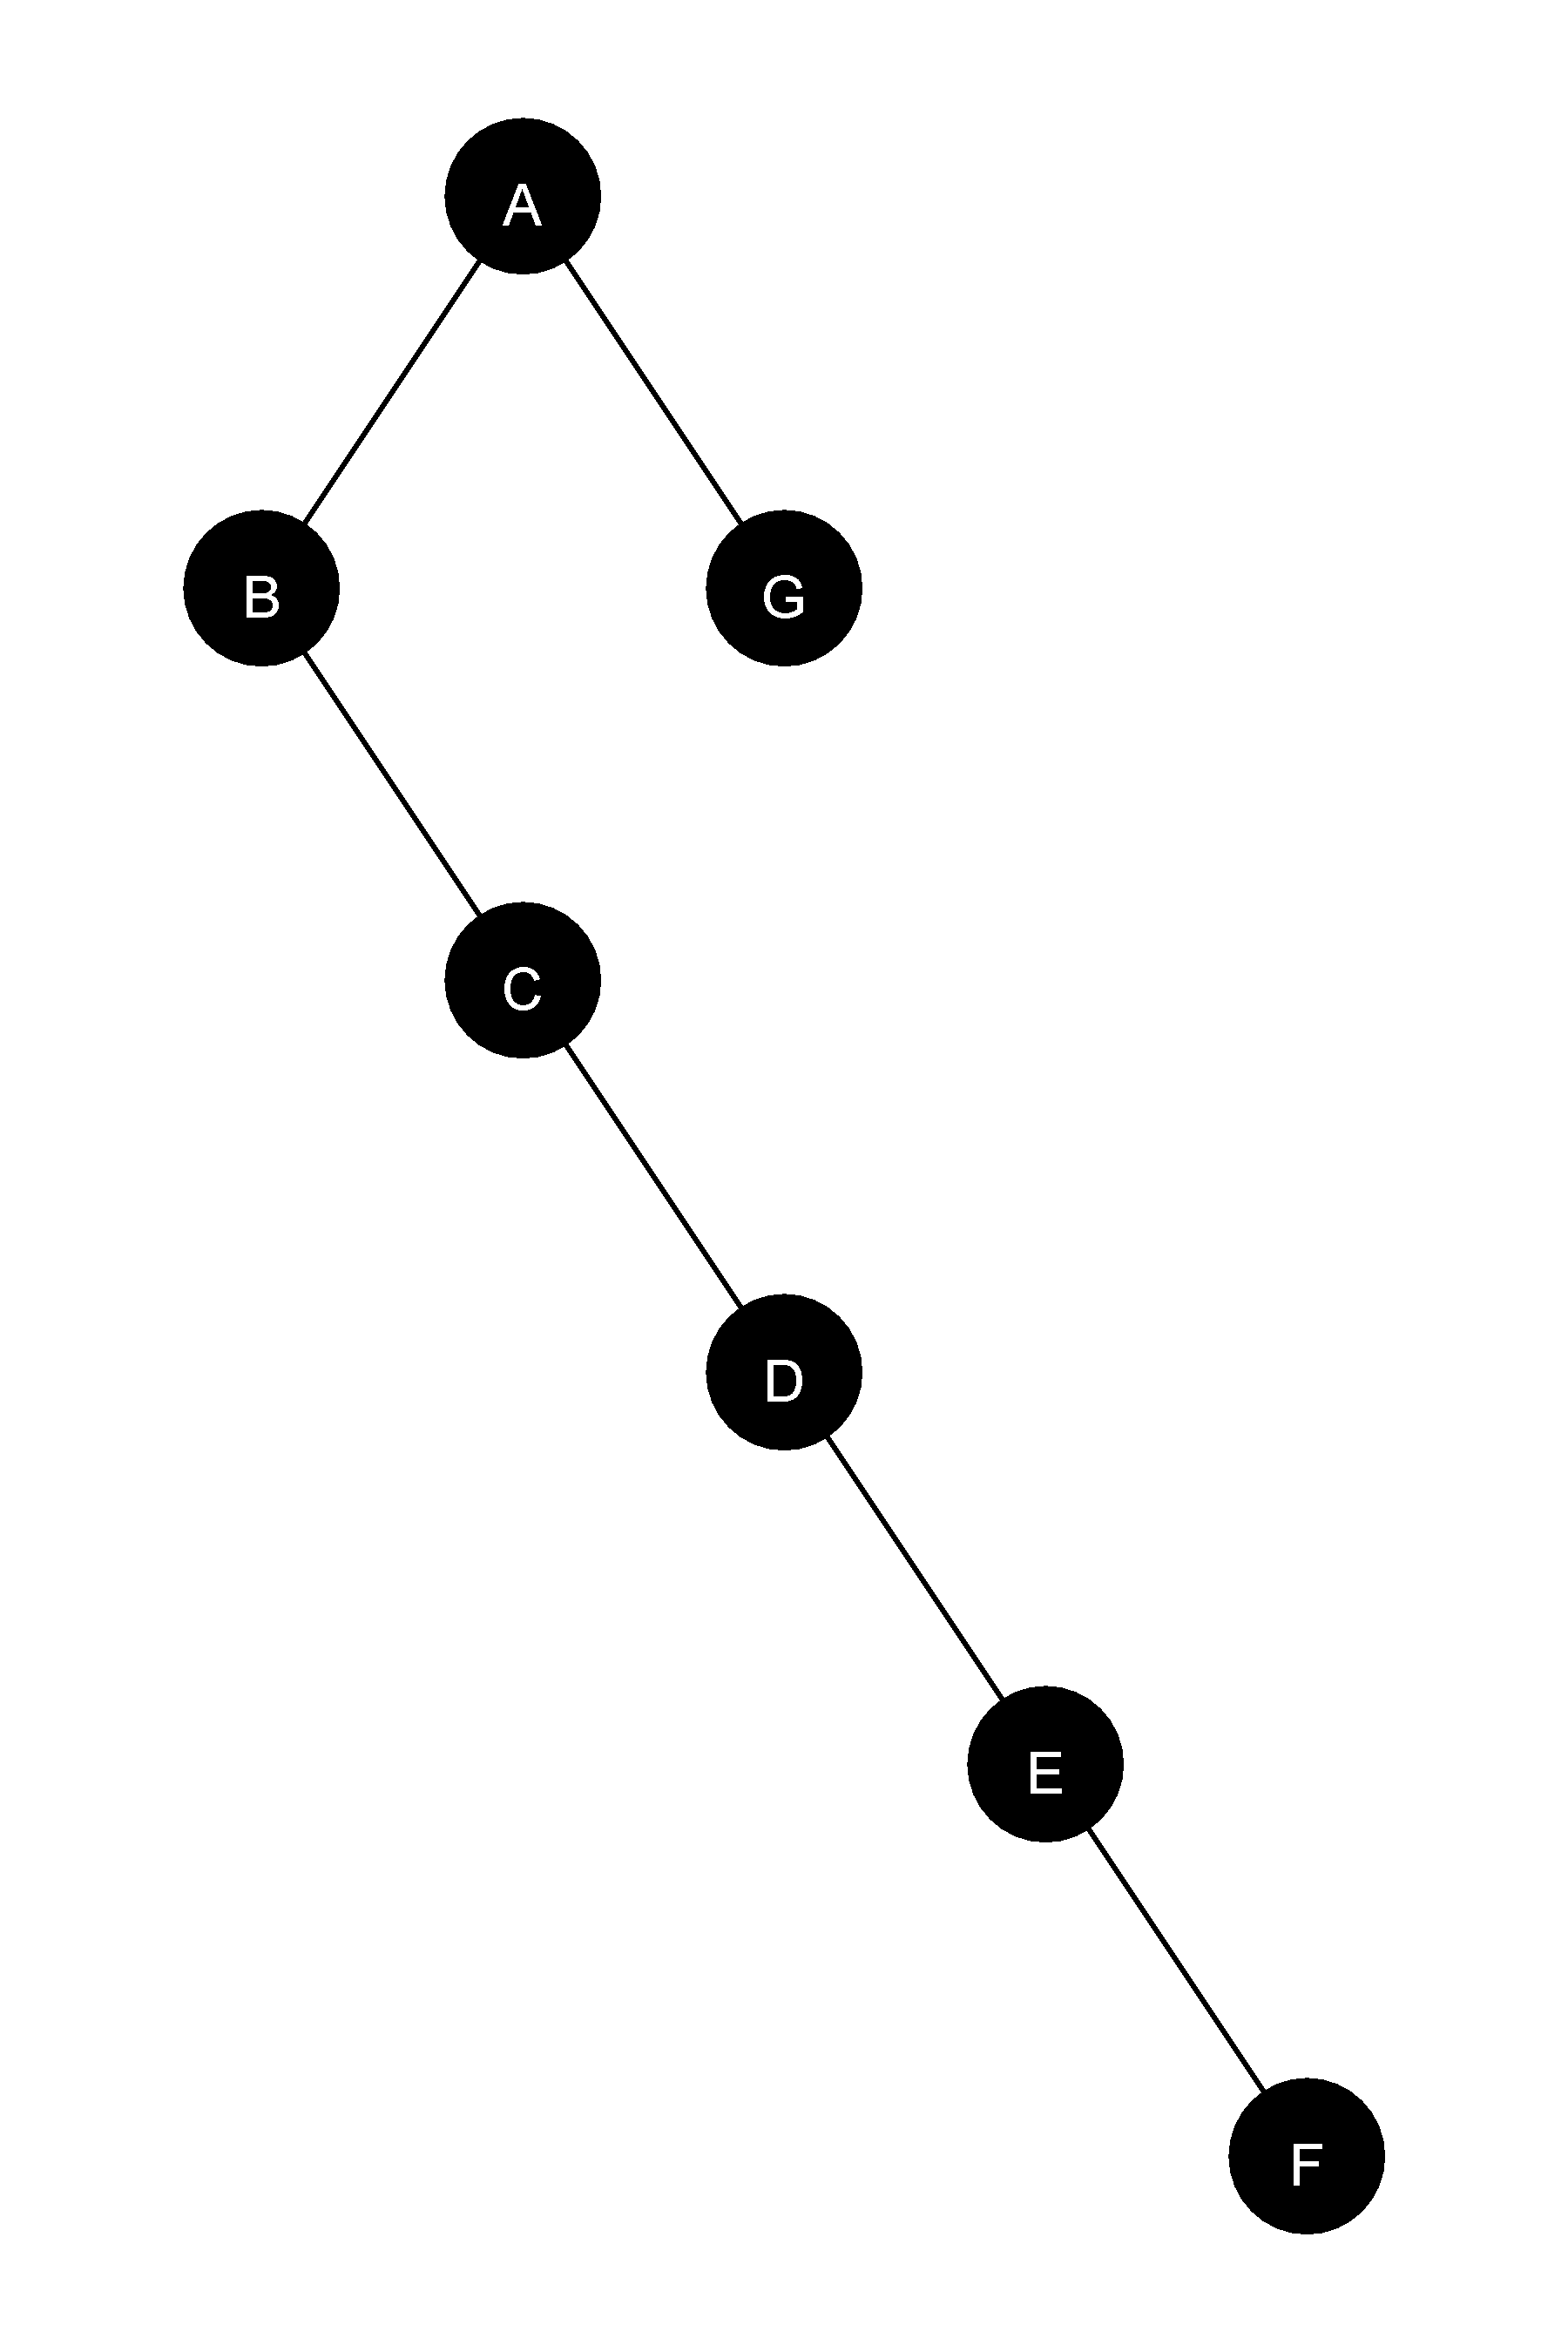
\includegraphics[scale = 0.06]{abbildungen/tree_spiegel_1_a2}
    \end{minipage}
    \hfill
    \begin{minipage}[t]{0.45\linewidth}
        \centering
        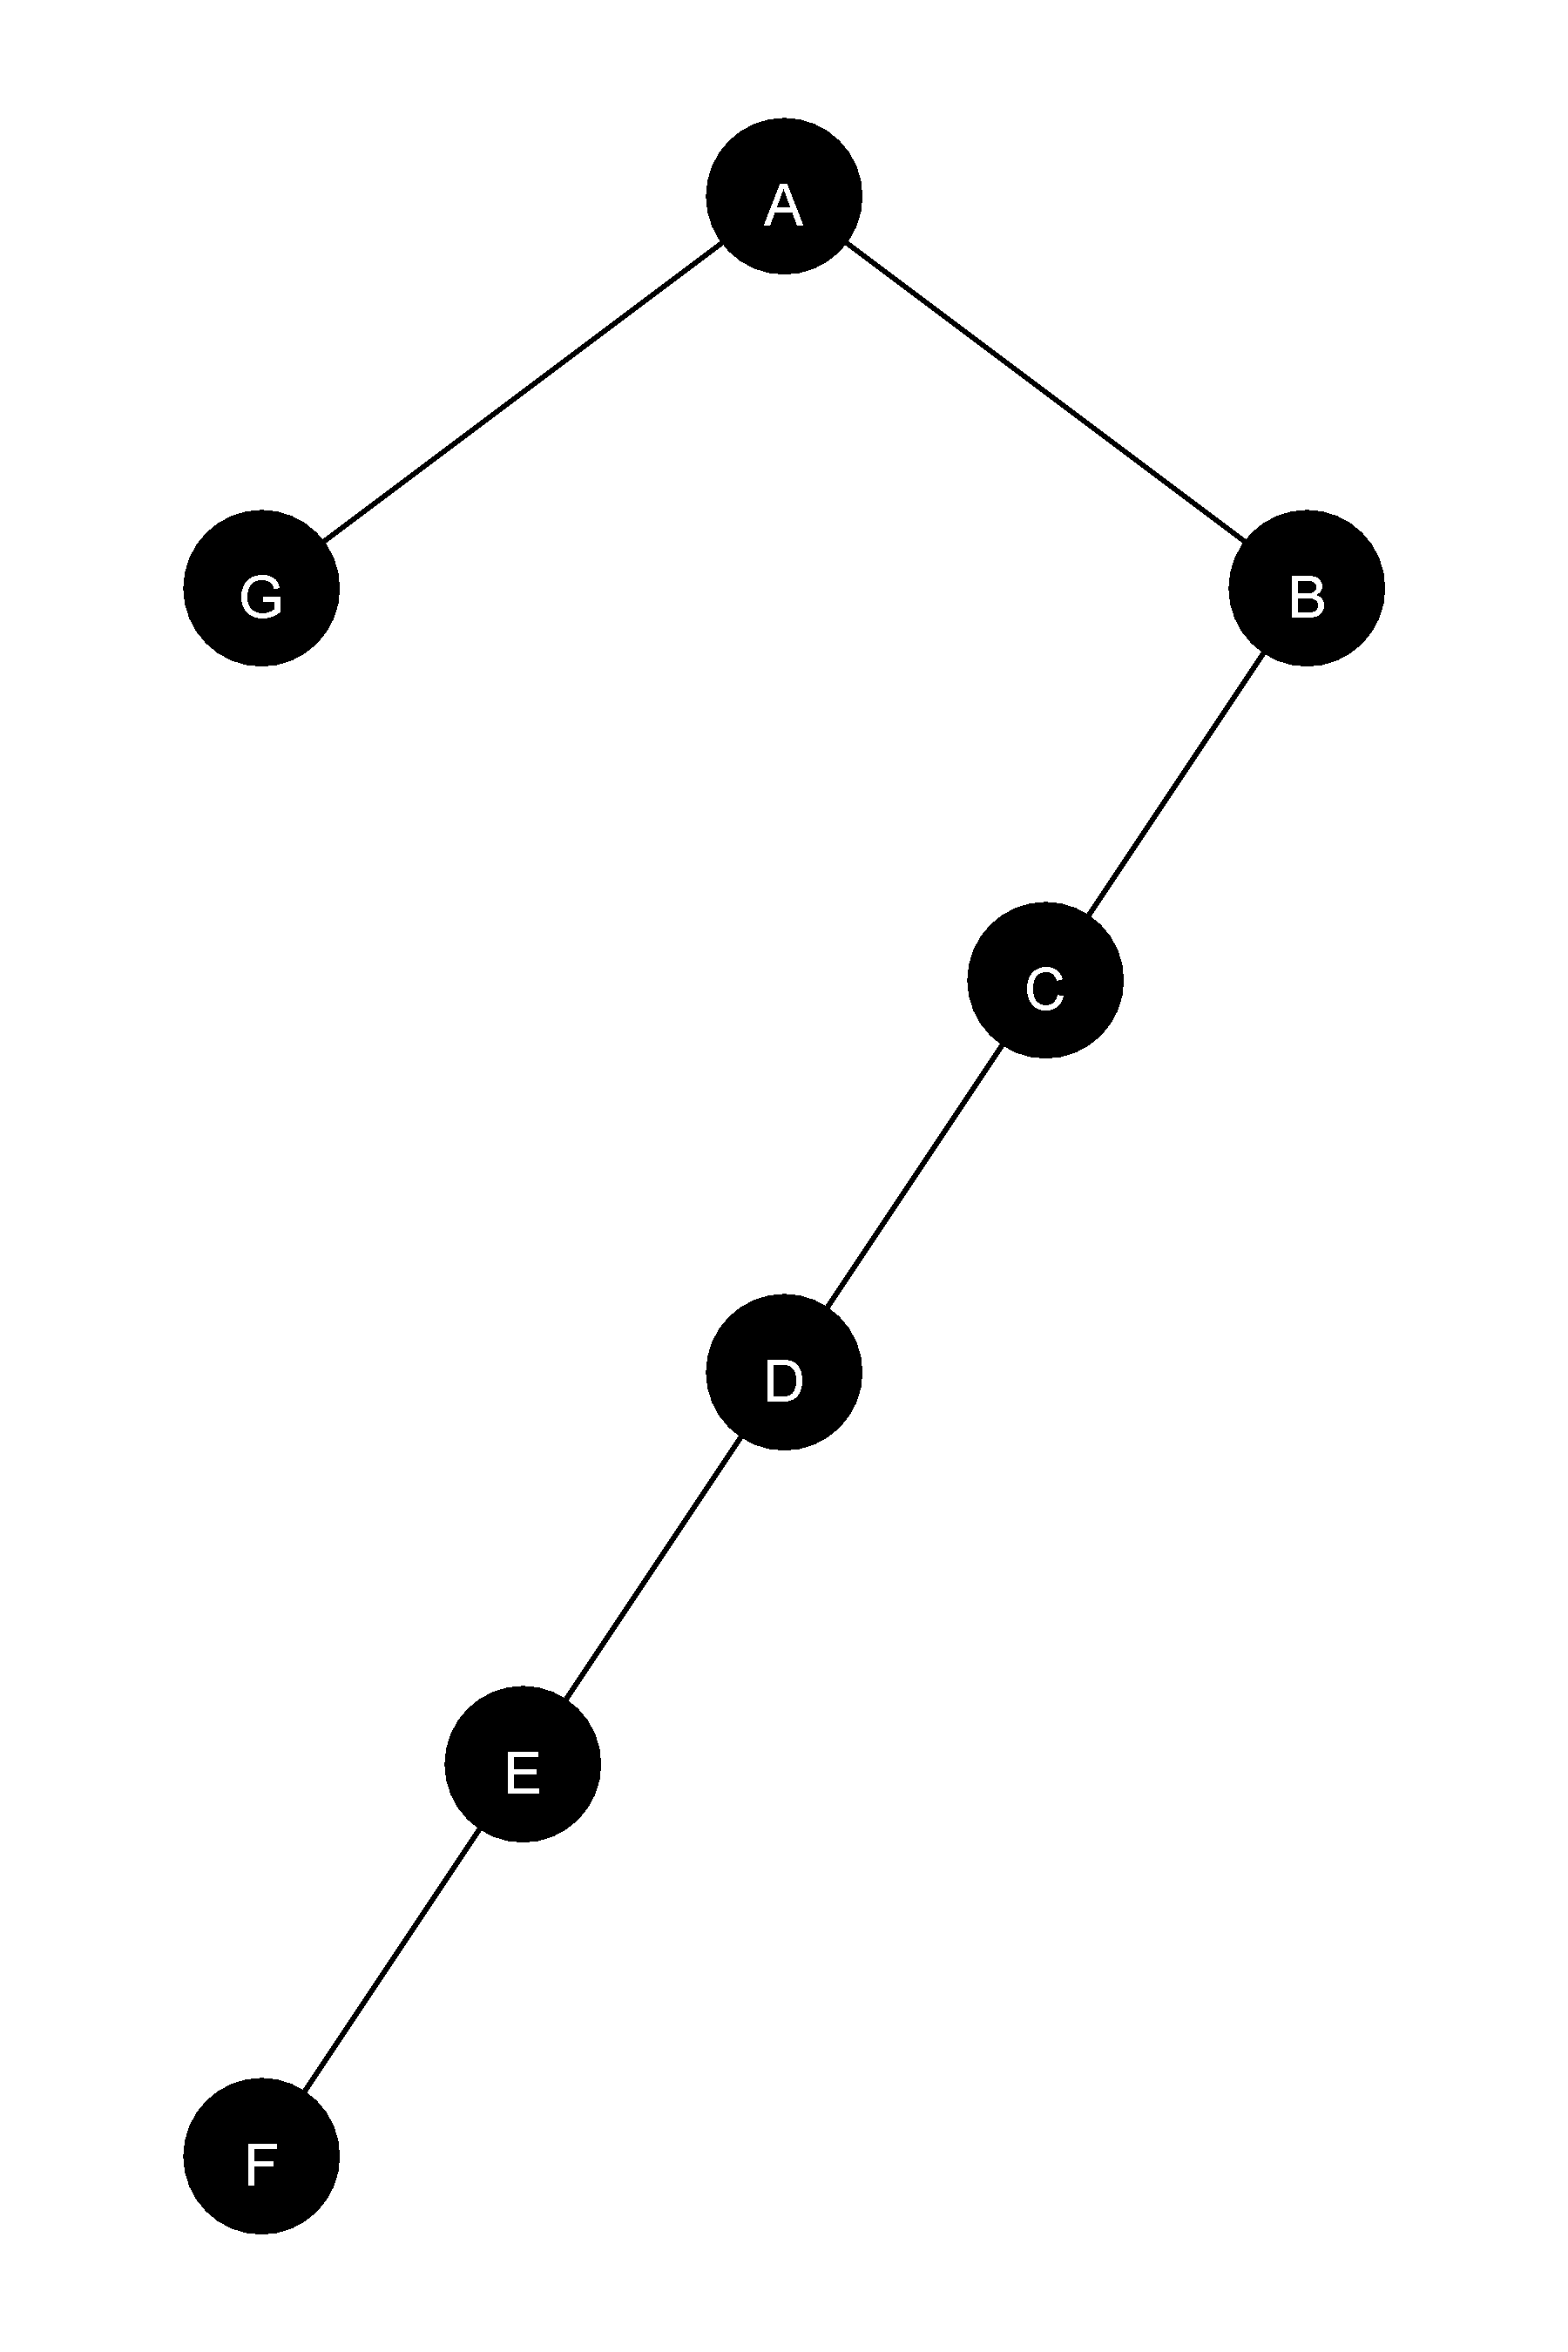
\includegraphics[scale = 0.06]{abbildungen/tree_spiegel_2_a2}
    \end{minipage} 
    \caption[]{Baum und Spiegelung gezeichnet nach WS}
    \label{pic:WS_Spiegel}
\end{figure}

\begin{figure}[ht]
    \centering
    \begin{minipage}[t]{0.45\linewidth}
        \centering
        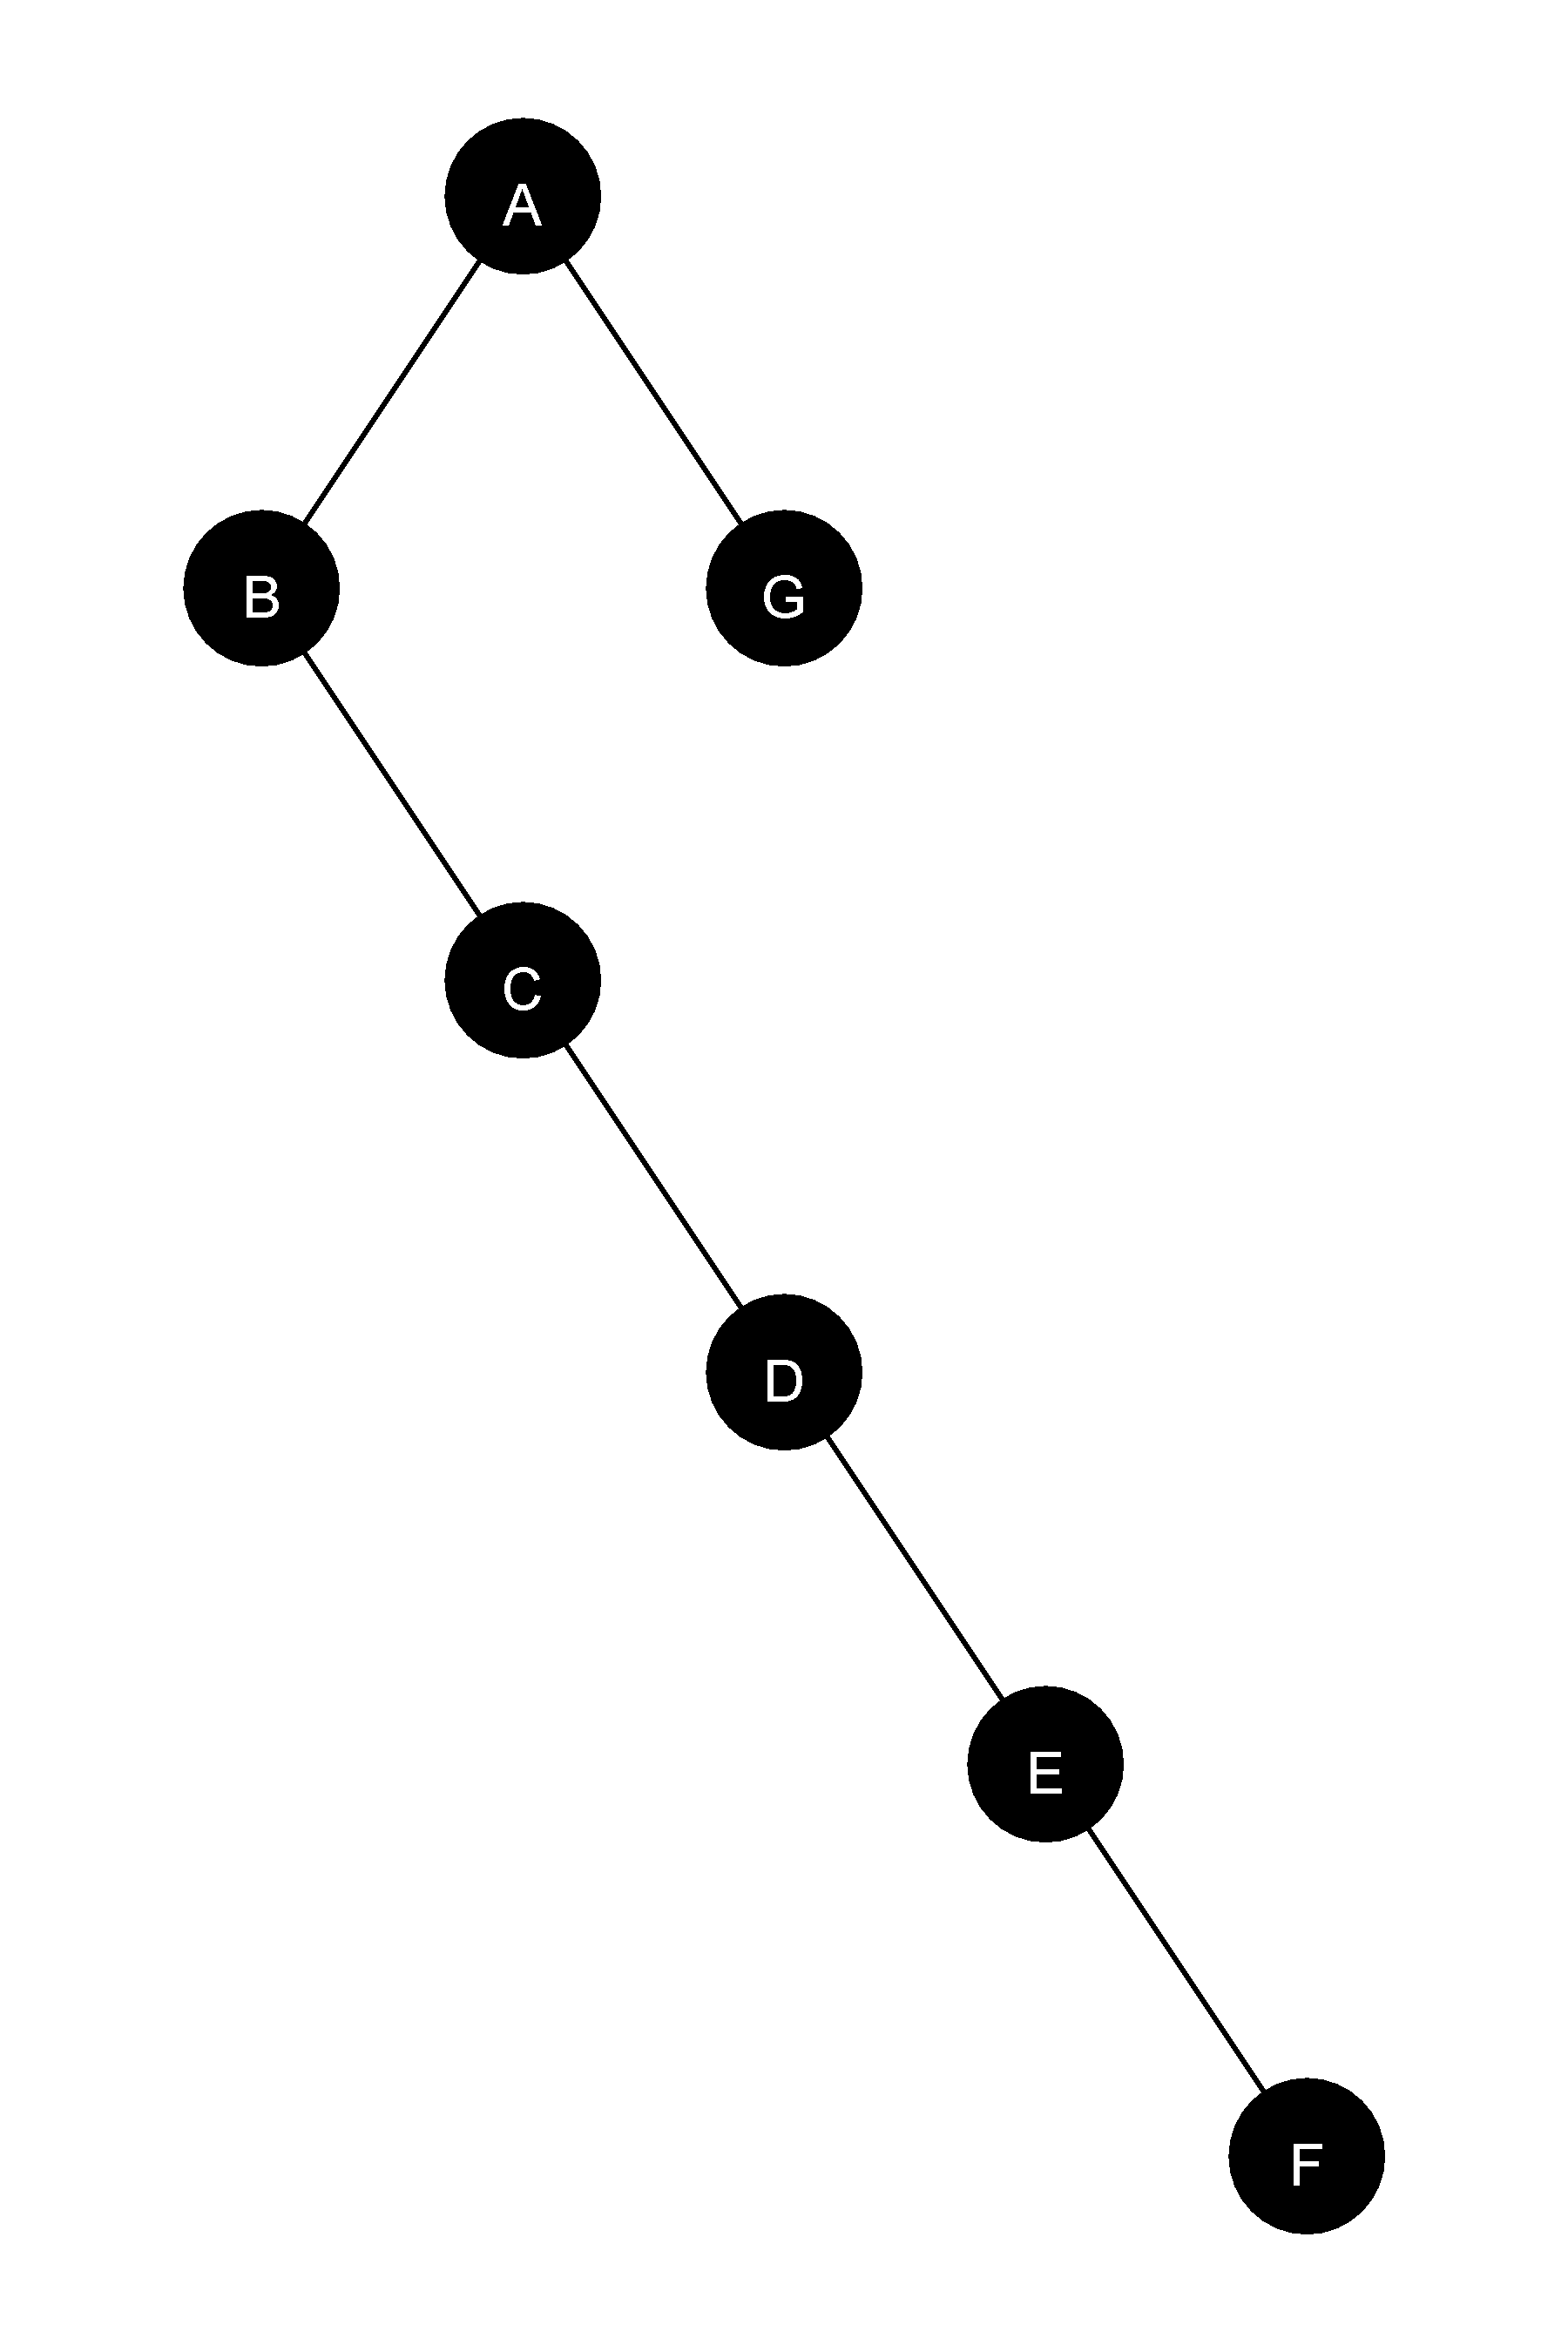
\includegraphics[scale = 0.06]{abbildungen/tree_spiegel_1_a3}
    \end{minipage}
    \hfill
    \begin{minipage}[t]{0.45\linewidth}
        \centering
        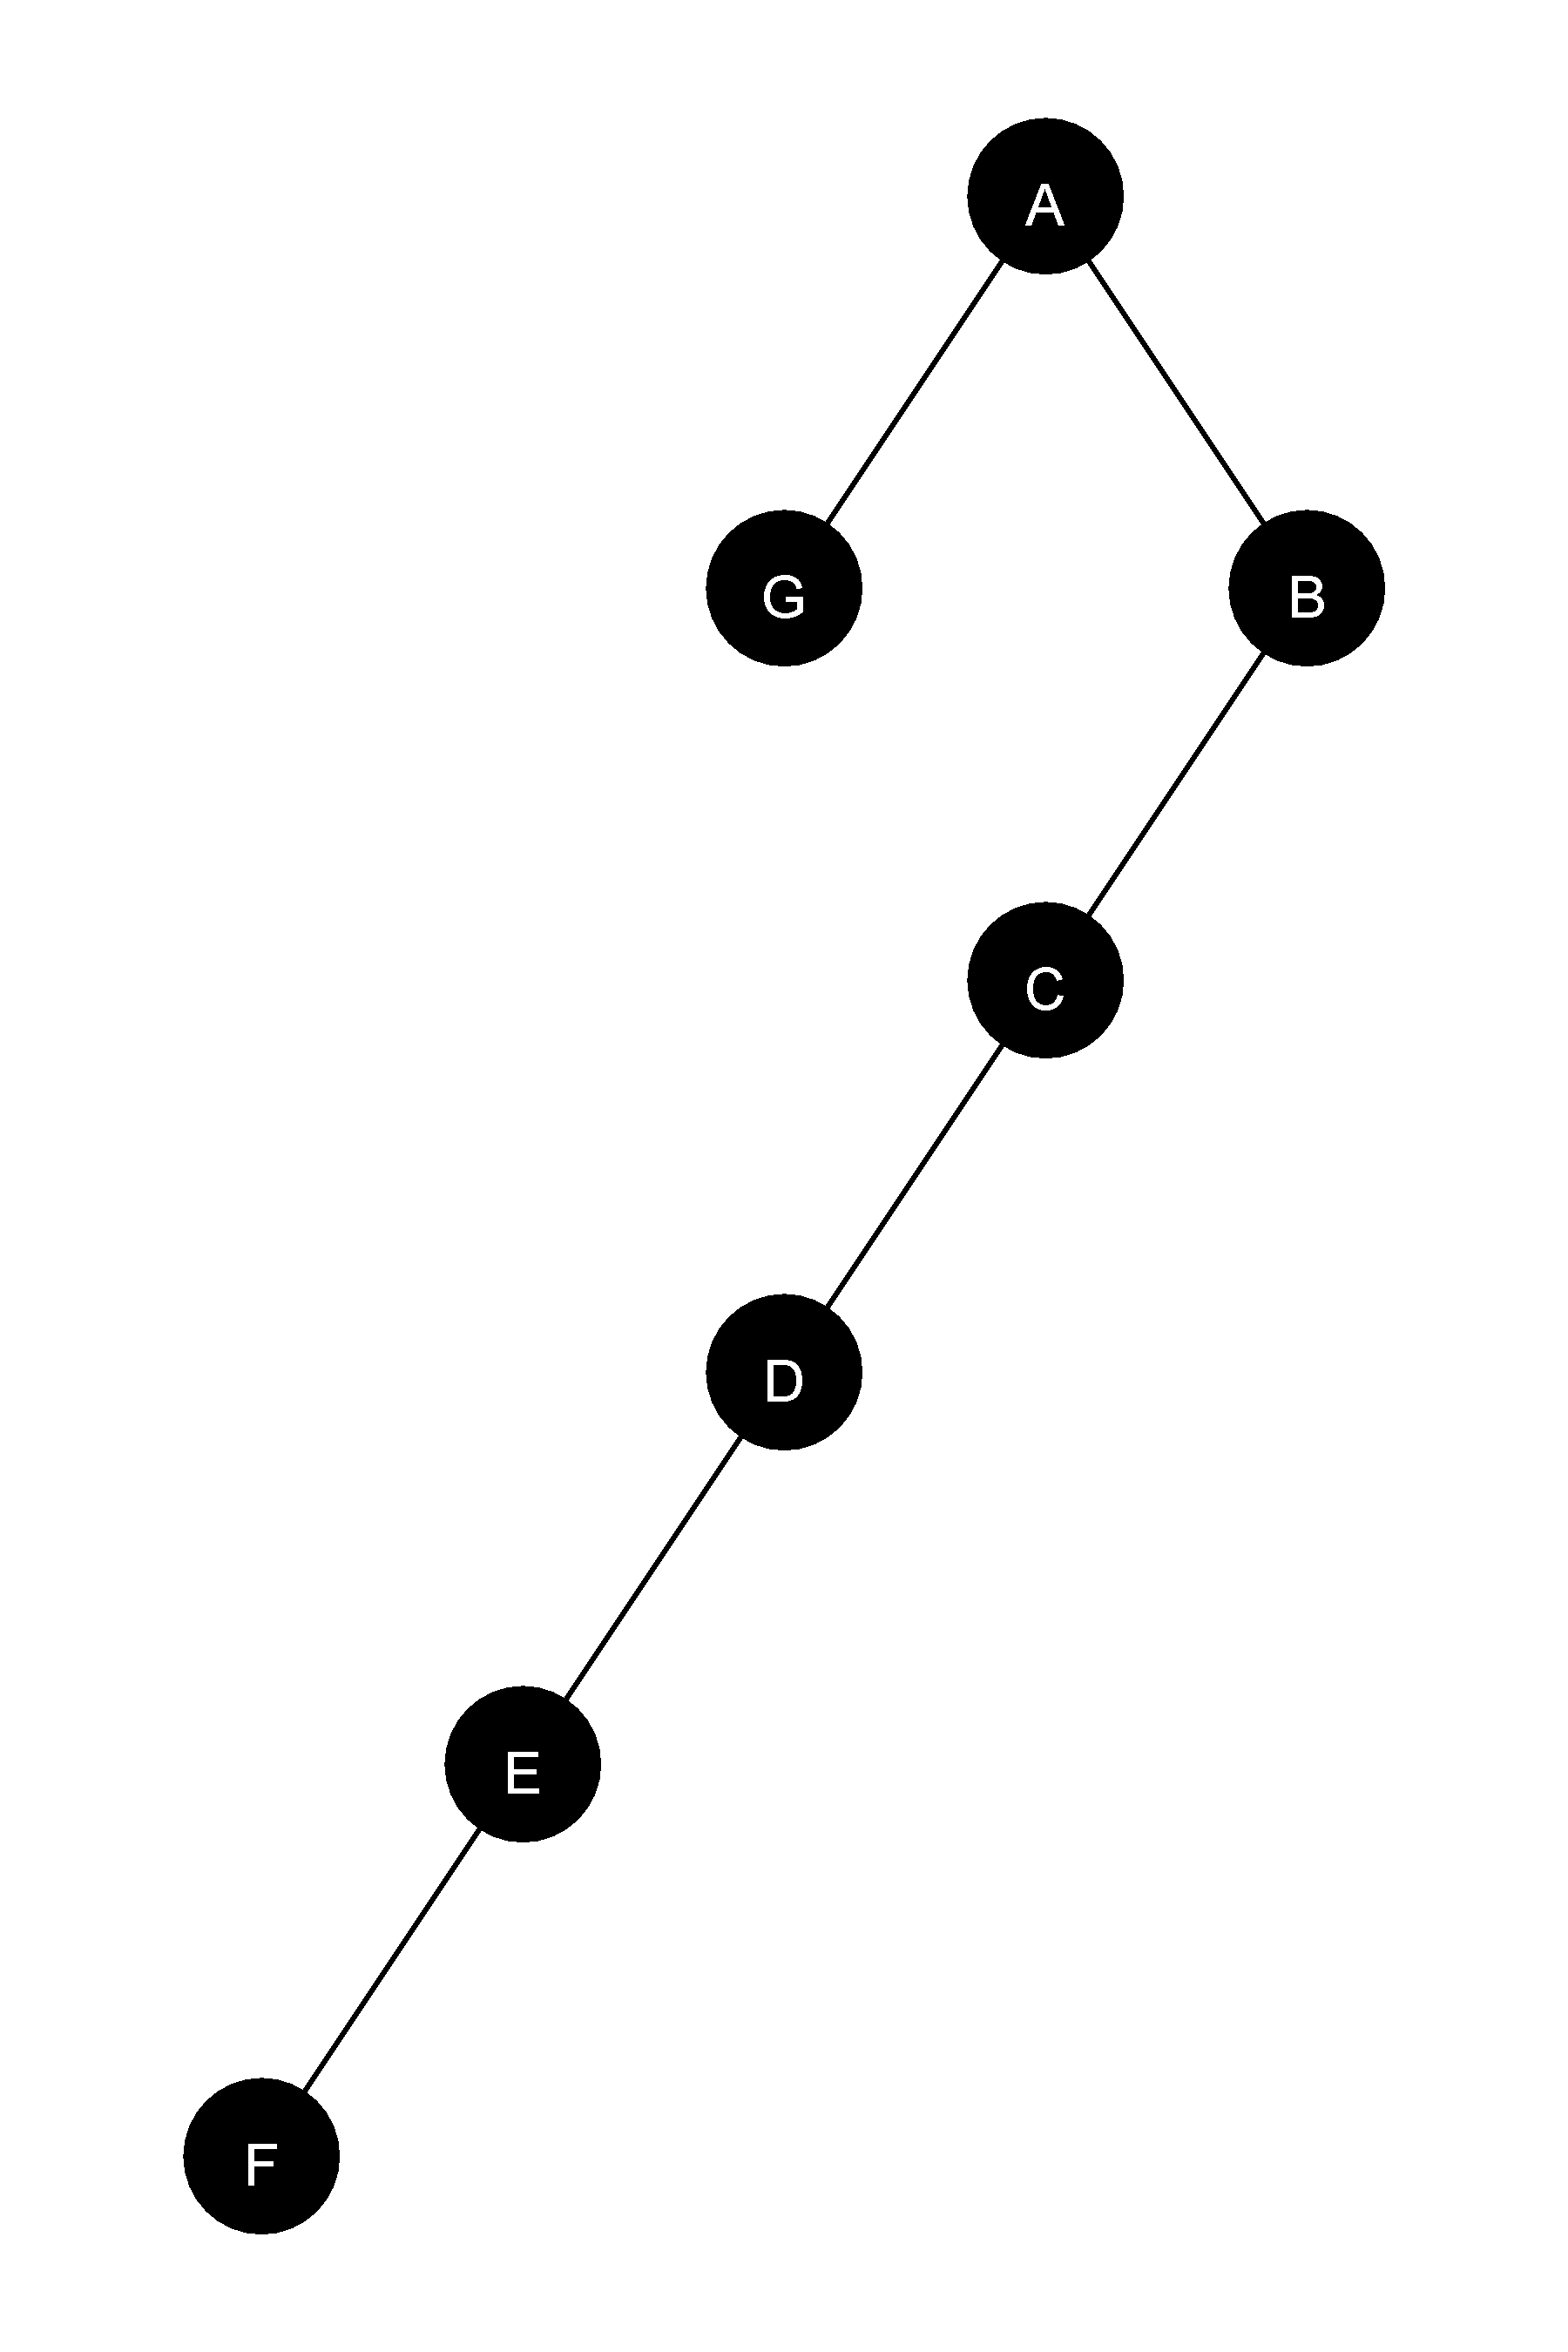
\includegraphics[scale = 0.06]{abbildungen/tree_spiegel_2_a3}   
    \end{minipage}  
    \caption[]{Baum und Spiegelung gezeichnet nach TR}
    \label{pic:TR_Spiegel}
\end{figure}

\chapter{Anhang B}
\label{chap:anhang_b}

\lstinputlisting[caption={Knoten-Klasse}]{abbildungen/git/src/algos/Knoten.java}

\lstinputlisting[caption={Binary-Klasse}]{abbildungen/git/src/algos/BinaryKnoten.java}

\lstinputlisting[caption={WS-Naiver-Algorithmus-Klasse}]{abbildungen/git/src/algos/NaiverAlgorithmus.java}

\lstinputlisting[caption={WS-Algorithmus-Klasse}]{abbildungen/git/src/algos/VerbesserterAlgorithmus.java}

\lstinputlisting[caption={RT-Algorithmus-Klasse}]{abbildungen/git/src/algos/TilfordAlgorithmus.java}

\lstinputlisting[caption={Zusatzklasse: Trees}]{abbildungen/git/src/algos/Trees.java}

\lstinputlisting[caption={Zusatzklasse: Drawer}]{abbildungen/git/src/algos/Drawer.java}

\lstinputlisting[caption={Zusatzklasse: Mains}]{abbildungen/git/src/algos/Mains.java}

% ***************************** BACK MATTER ***********************************
%\thispagestyle{empty}

%\addcontentsline{toc}{chapter}{\protect\numberline{}Eidesstattliche Erklärung}
%\chapter*{}
\vspace*{0.5cm}
\noindent

Hiermit versicheren wir, dass wir die vorliegende Arbeit selbstständig verfasst und keine anderen als die angegebenen Quellen und Hilfsmittel benutzt haben. Wir versicheren, dass wir alle wörtlich oder sinngemäß aus anderen Werken übernommenen Aussagen als solche gekennzeichnet haben, und dass die eingereichte Arbeit weder vollständig noch in wesentlichen Teilen Gegenstand eines anderen Prüfungsverfahrens gewesen ist.

\vspace{3cm}
\toponym, den \today

\end{document}